\documentclass{standalone}

\usepackage{tikz}
\usetikzlibrary{positioning, arrows, shapes, calc, plotmarks, backgrounds, fit}

\begin{document}
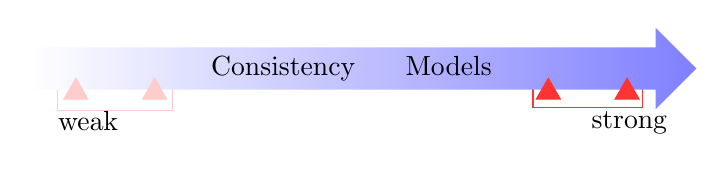
\begin{tikzpicture}

    \node (consistency-models-bar) [single arrow, text width = 8cm, align=center, 
    shade,shading=axis, left color=white,right color=blue!50, inner sep = 3pt] {Consistency 
    $\;$  Models}; 

    \node (weak) [mark size = 5pt, color = red!20] at (-3.5cm, -0.3cm) {\pgfuseplotmark{triangle*}};
    \node (weak-right) [mark size = 5pt, color = red!20] at (-2.5cm, -0.3cm) {\pgfuseplotmark{triangle*}};
    \node (weak-text) [below right = 0.0cm and -0.35cm of weak.south] {weak};
    
    \node (strong) [mark size = 5pt, color = red!80] at (3.5cm, -0.3cm) {\pgfuseplotmark{triangle*}};
    \node (strong-left) [mark size = 5pt, color = red!80] at (2.5cm, -0.3cm) {\pgfuseplotmark{triangle*}};
    \node (strong-text) [below right = 0.0cm and -0.70cm of strong] {strong};

    \begin{pgfonlayer}{background}
      \node (quantify-weak) [draw = red!20, fit = (weak) (weak-right), inner sep = 3pt, rectangle] {};
      \node (weaken-strong) [draw = red!80, fit = (strong) (strong-left), inner sep = 2pt, rectangle] {};
    \end{pgfonlayer}
    
\end{tikzpicture}
\end{document}
